\documentclass[msc, oldfontcommands]{ppgccufmg} %

\usepackage[english]{babel} %

\usepackage{algorithm}
\usepackage{algpseudocode}
\usepackage{multirow}

\usepackage[T1]{fontenc}
\usepackage[utf8]{inputenc}

\usepackage{graphicx}
\usepackage[square]{natbib}
\usepackage{array, makecell} %

\usepackage{multirow}

\begin{document}

\ppgccufmg{
title={Protocol for Error-Verification inside\\Totally Error-Free
Networks},
authorrev={da Camara Neto, Vilar Fiuza},
university={Federal University of Minas Gerais},
course={Computer Science},
portuguesetitle={Protocolo para Verificação de Erros\\em Redes
Totalmente Confiáveis},
portugueseuniversity={Universidade Federal de Minas Gerais},
portuguesecourse={Ciência da Computação},
address={Belo Horizonte},
date={2005-01},
advisor={Adamastor Pompeu Setúbal},
%approval={img/approvalsheet.eps},
%abstract=[brazil]{Resumo}{resumo},
%abstract={Abstract}{abstract},
%dedication={dedicatoria},
%ack={agradecimentos},
%epigraphtext={Truth and lie are opposite things.}{Unknown},
keywords={ola}
}

\chapter{Introduction}
\label{sec:intro}

The amount of multimedia data currently available is immense and is growing at an unprecedented rate. For instance, more than five hundred hours of video are uploaded every minute on YouTube. Detailed metadata of multimedia data, such as music, video, and images, is typically not available because of the cost and the hard task of meaningfully describing these objects. This problem can be addressed by representing multimedia objects using high-dimensional feature vectors or descriptors (100-1000+ dimensions) automatically computed~\cite{Wan:2014:DLC:2647868.2654948,10.1007/978-3-319-10584-0_26,Douze:2009:EGD:1646396.1646421}. 

Searching in these databases, such as performed by content-based multimedia retrieval (CBMR) services, is a fundamental operation for several multimedia applications~\cite{Bohm2001322}. Although similarity search may involve several steps, the most time consuming consists in finding the k nearest neighbors (k-NN) of a query object descriptor(s) in the database. 

The exhaustive exact search is costly due to, not only the large databases currently used by web applications, but also due to the high dimensionality of the descriptors. An alternative to the exhaustive search would be to employ data structures, such as kd-trees~\cite{Friedman1977209} and k-means trees~\cite{Muja2009331}, to partition the space and efficiently prune data partitions during the search. However, the pruning efficiency and, consequently, the performance of these techniques, degrade as the data dimensionality grows due to the well known curse of dimensionality~\cite{Weber:1998:QAP:645924.671192}. 

The approximate nearest neighbors (ANN) search has been proposed as a solution for those applications in which the exact search is not strictly necessary, allowing for accuracy to be traded off for speed. Thus, a large number of ANN algorithms have been developed~\cite{Gionis:1999:SSH:645925.671516,5432202,NIPS2009_3864,6809191,Muja2009331}. The product quantization nearest neighbor search (also known as IVFADC)~\cite{5432202} has received special attention among competitors due to its ability to minimize memory requirements, while improving speed. This is attained by representing descriptors with small quantization codes and by using an inverted list to avoid exhaustive search in the quantized space. It was recently ported for GPU~\cite{8733051}.

Most of the previous work, however, has focused on optimizing those algorithms for batch execution using sequential settings or a single machine. This decision does not match the demands of modern online CBMR services, which must handle very large and increasing databases that would not fit in the memory of a single machine. Also, while online applications are concerned with minimizing the query response times of individual queries ($query\ response\ time\ =\ queue\ waiting\ time + processing\ time$), the aforementioned algorithms were developed to maximize throughput in a batch execution where several queries are bundled and processed together as a single task. The online scenario presents additional challenges because these systems experience fluctuating workloads, and must adapt to them at run-time to minimize response times. 

In our setting the adaptation is performed in the number of queries (query block size) dispatched for execution with the GPU in each device call. For instance, when the input query rates are low, the queue waiting
time is negligible, and minimizing the processing time is the best approach. This is attained by reducing the query block size
so that more computing resources or core in the GPU are assigned to process each query, thus reducing the processing time of that block of queries. However, as the system load increases, the queue waiting time grows and the system should be configured to improve
the throughput to minimize congesting in queue of queries ready to execute. This is attained by increasing the query block size or number of queries concurrently executed with the GPU. The larger number of queries processed executed concurrently 
improves the throughput because of the reduction on synchronization overheads in a query computation (smaller number of
cores assigned to it) and the best amortized communication and startup overheads.

%few queries can be bundled for GPU execution and, consequently, more resource %is available to process each of them. When the load increases, however, the %system throughput must be improved to avoid congestion in the queue of queries %waiting to be executed. This is attained by bundling a larger number of %queries for concurrent execution with the GPU, which will attain higher %efficiency because of the lower synchronization costs due to the smaller %number of GPU cores assigned to a query and because of the amortized costs of %launching the computation in the GPU. Dealing with this variation is %fundamental for delivering the best response times in all scenarios.

This work addresses these challenges with a distributed-memory parallelization of IVFADC targeting hybrid machines equipped with CPUs and GPUs. The proposed parallelization avoids data replication and allows for large databases to be searched. Besides, a carefully designed asynchronous communication is performed to minimize overheads. We have also developed multiple strategies to execute query searches using CPU and GPU cooperatively. Even though the GPU can typically reach much higher query processing rates, the CPU is able to significantly reduce the query response times under several query load configurations. We also proposed an out-of-core GPU execution in which the GPU is efficiently used  
when the database index does not fit into its memory. In this setting, the GPU may also be used in cooperation with the CPU, and work stealing is employed to minimize the load imbalance among the devices. 

This paper makes the following major contributions:

\begin{itemize}
    \item We implement an efficient distributed memory version of IVFADC for hybrid CPU-GPU systems. The execution on a CPU-GPU machine can answer 6364 queries/sec on a single node, and its distributed execution scaled with an efficiency of YYY on ZZZ GPUs-CPUs.
    
    \item We have developed the DQPP strategy for adjusting the system at run-time under fluctuating workloads, which decides the number of queries for concurrent execution with the GPU according with the system load. DQPP improved response times vs. the best static approach in 1.29$\times$ and 1.35$\times$, respectively, for the GPU-only and CPU-GPU configurations with moderate loads.
    
    \item We implemented an out-of-core GPU execution scheme that uses work-stealing for maximizing performance on the CPU-GPU cooperative. The CPU-GPU execution with work stealing improved the throughput and response times vs. the GPU-only execution, respectively, in 1.26$\times$ and 2.4$\times$. 
    
\end{itemize}

The remainder of this manuscript is organized as follows: Section~\ref{sec:back} presents a background on high-dimensional similarity search. Section~\ref{sec:pqnns} details the product quantization nearest neighbor search. Section~\ref{sec:parallel} presents the IVFADC parallelization on distributed memory and hybrid CPU-GPU equipped machines and details optimizations to deal with out-of-core GPU execution. The response time aspects are further presented in Section~\ref{sec:query-rate-aware}. Finally, the experimental results are discussed in Section~\ref{sec:experimental-results}, and our conclusions are in Section~\ref{sec:conclusions}.
\chapter{Background}
\label{sec:back}

Similarity search is a fundamental operation found in Content-Based Multimedia Retrieval (CBMR). In multimedia retrieval, the documents are embedded into a multi-dimensional space using descriptors, which intend to bridge the ``semantic gap" between the low-level coding  representing the documents and their semantic concepts. The search is then performed in the descriptors space by using a distance metric (e.g., Euclidean distance) to represent the similarity between a query and the database descriptors. 

Several descriptors have been evaluated in the literature. They capture different properties of the data, such as color, texture, shape, and orientation; and are encoded into high-dimensional feature vectors. Some of the most popular descriptors are Scale Invariant Feature Transform (SIFT), Gist, Bag-of-Features (BOW), Vector of Locally Aggregated Descriptors (VLAD) and deep features~\cite{Wan:2014:DLC:2647868.2654948,10.1007/978-3-319-10584-0_26,Douze:2009:EGD:1646396.1646421}. Regardless of the descriptor used, the similarity search is a major time consuming phase of most multimedia applications.

\section{Similarity Search Algorithms}

Given a descriptor query, the similarity search refers to finding the closest k nearest neighbor (k-NN) descriptors in the database. The exact brute force algorithm for this operation computes the distance from the query descriptor to each descriptor in the database, and selects the closest k ones. This is, however, prohibitive for online multimedia services. 

In order to reduce the cost of the exact k-NN, several data structures (e.g., kd-trees~\cite{Friedman1977209}, k-means trees~\cite{Muja2009331}, ball trees~\cite{UHLMANN1991175}, and cover trees~\cite{Beygelzimer:2006:CTN:1143844.1143857}) were used to divide the database of descriptors into partitions according to their spatial location. This organization is intended to prune partitions during the search phase and, consequently, speed it up. However, because of the well known  ``curse of dimensionality''~\cite{Bohm2001322,Weber:1998:QAP:645924.671192}, the sparsity of the data quickly increases as the data dimensionality grows. This reduces the pruning efficiency of those data structures and, as a consequence, their performance improvements vs. the brute force search.

Due to the the high cost of computing the exact k-NN, the approximate nearest neighbors (ANN) search has been proposed for applications in which the exact solution is not essential. The approximation in this case may be bound by the number of missing correct descriptors or their distance to the query~\cite{Indyk:1998:ANN:276698.276876}. Even on the ANN case, efficiently searching large databases remains a very challenging problem.

Several ANN methods have been proposed~\cite{Gionis:1999:SSH:645925.671516,5432202,NIPS2009_3864,6809191,Muja2009331}. The locality sensitive hashing (LSH) uses locality sensitive hashing functions to index data into multiple hash tables. Descriptors in a hash entry, or bucket, are expected to be close in the multi-dimensional space. The search visits buckets to which the query is hashed, the distances to descriptors on those buckets are computed, and the nearest neighbors from that subset will compose the query answer. The tuning of LSH parameters leads to several hash tables, which poses a scalability challenge with large databases due to high memory demands. Also, modern machines have a low random memory access performance~\cite{TeodoroKKCS14}, which is a major pattern in LSH during hash table buckets visits. 

The fast library for approximate nearest neighbors (FLANN) is a popular open source project for ANN search. It implements multiple state-of-the-art algorithms and selects the most appropriate along with its parameters for a given dataset. This alleviates the hard and error-prone task of choosing from the several indexing approaches
available. 
%It also shows that a single approach will not be efficient in all cases~\cite{Muja2009331}.
It also shows that there is no one-size-fits-all solution for ANN search~\cite{Muja2009331}. Because of its efficiency, FLANN is typically used as a baseline for performance comparisons.

The product quantization based nearest neighbor search is another approach to the problem~\cite{5432202}. 
It divides the high-dimensional multimedia descriptor vectors into low dimensional subspaces, 
and quantizes the subspaces independently. Two quantization phases are used, the first 
called coarse and the second to quantize residuals from the first. The 
coarse quantization is used to assign objects to entries of an inverted file, whereas 
the second compresses residual distances to the coarse quantizers. This results 
in the IVFADC indexing, which has been shown to be very competitive as
compared to the previous works~\cite{5432202}. 

Because of its efficiency, we have parallelized IVFADC 
for distributed systems equipped with CPU and GPU (Section~\ref{sec:pqnns}). There have been proposed improvements to the IVFADC in the literature
with the multi-index~\cite{6915715} that depends on a complex index visiting sequence, LOPQ~\cite{6909695}, and Polysemous codes~\cite{978-3-319-46475-6_48}. However, as discussed in~\cite{8733051}, these estrategies are not appropriate for GPU implementation. As a consequence,
the current state-of-the-art ANN implementation for GPUs is based on IVFADC~\cite{8733051}.
Furthermore, despite choosing IVFADC for our parallelization and optimizations, we argue that the proposed
approaches for dealing with varying workloads, the distributed-memory parallelization strategy, and
the optimizations for processing GPU out-of-core databases can benefit other indexing algorithms.

\section{Parallel Similarity Search}

Although most of the ANN research has focused on optimizing the speed and
quality of sequential algorithms, this is changing because of 
current demands for indexing very large databases. Multiple works have  evaluated
multi-core CPUs, GPUs, and distributed memory machines to perform large-scale multimedia similarity search~\cite{2398596,Stupar10rankreduce,Moise:2013,8733051,6267877,Krulis2012,7780592,6809191,2093973.2094002,Teodoro2014,ANDRADE201981}.

Distributed memory implementations of LSH were developed on top of MapReduce~\cite{2398596,Stupar10rankreduce}. 
%In both cases, a $map\ phase$ is employed to visit multiple hash buckets, whereas the $reduce\ phase$ 
%aggregates local results returned by the map operations. 
The approach of Stupar 
et al.~\cite{Stupar10rankreduce} stores the data into a distributed file system. Because LSH may require several 
hash tables, the data is replicated in each of the tables. This 
increases the query latency and reduces efficiency, making this solution 
impractical for large databases~\cite{Stupar10rankreduce}. Bahmani et al.~\cite{2398596} implemented a variant of the 
LSH using an Active Distributed Hash Table (DHT) to store the database in memory, and it assumes that a single LSH hash table is 
instantiated. In this case, multiple queries to the LSH table are required to attain the desired search quality as performed by 
multi-probe LSH~\cite{1325958}, but it is not evaluated. Another relevant work~\cite{Moise:2013} 
has discussed the deployment of the Index Tree on top of MapReduce. This work has
implemented a full search engine in a distributed memory system and discussed the technical 
challenges in this process. Similarly to the previous works, this solution is optimized 
for batch processing only. %FLANN~\cite{6809191} proposed a distributed memory parallelization based on the master-slave model in which
%the indexing scheme is instantiated into several nodes and the input data is partitioned among them. Their 
%execution, as discussed in~\cite{6809191}, suffers from high memory demands due to the algorithms implemented, 
%limiting the scalability for large datasets.
% Im not sure if this is allowed
In a previous work~\cite{ANDRADE201981}, we have implemented a distributed memory IVFADC 
that executes on CPU-only machines. It is extended in this paper in multiple directions. Here, we proposed and implemented (i)~the use
of GPUs in the distributed memory execution; (ii)~the cooperative
execution on hybrid systems equipped with CPU-GPU; (iii)~new algorithms for adjusting the GPU search
with the goal of minimizing response times; (iv)~an out-of-core GPU execution to process databases
larger than the GPU memory; (v)~optimizations to minimize load 
imbalance between CPU and GPU with the use of work stealing.

The use of GPUs has been evaluated on shared memory systems~\cite{8733051,6267877,Krulis2012,7780592,2093973.2094002}. Among these works, the ones that
implemented the IVFADC~\cite{7780592,8733051} have attained the best trade-off with respect to the search quality and 
throughput. These implementations have been compared and the~\cite{8733051} 
has attained the 
best performance.
%As such, in this work, we leveraged that GPU implementation, adapted, and used it as a basic building block of our distributed 
%memory implementation.
In this work, it is used as a basic building of our distributed memory implementation.
\chapter{Product quantization ANN search}
\label{sec:pqnns}

This section presents the product quantization, its use in nearest 
neighbor search, the indexing structure employed in the search~\cite{5432202},
and the single node GPU IVFADC~\cite{8733051}.

\section{Product quantization}

Quantization is a process for reducing the cardinality of the representation space. Considering 
a $D$-dimensional vector $x$, a quantizer is a function $q$ that maps $x$ into a 
vector $q(x) \in C = {c_i;i\in L}$, with the index set $L$ of finite size $0 \ldots k-1$. 
The $c_i$ values are called centroids and $C$ is the codebook. The effective quantization
of high-dimensional vectors in this framework would require a large codebook to 
minimize the quantization error~\cite{5432202}. This is, however, impractical because of the 
high quantization cost and the memory required.
%to store C.

The product quantization has been proposed to address these issues. In this technique, 
the vector $x$ is split into $m$ disjoint subvectors $u_j$ ($j \in 1...m)$ with $D^*=D/m$ 
dimensions, assuming $D$ multiple of $m$. Each $x$ is quantized as follows:

\begin{equation}
\small
\underbrace{x_1,...,x_{D^{*}}}_{u_1(x)},...,\underbrace{x_{D-D^{*}+1},...,x_D}_{u_m(x)} \rightarrow q_1(u_1(x)),...,q_m(u_m(x))
\end{equation} 

This results in quantizing $x$ through a Cartesian product of its quantized subvectors:

\begin{equation}\label{eq:subquant}
q(y) = q_1(u_1) \times q_2(u_2) \times ... \times q_m(u_m)
\end{equation}

This process creates large codebooks by using low-complexity quantizers 
in subvectors. The quantized vectors are represented by a composition of
subvector quantization indices ($\tau = \tau_1 \times \ldots \times \tau_m$), leading
to a codebook $C = C_1 \times \ldots \times C_m$ with $C_j$ being the centroids 
used for each subvector quantization. Assuming that $k$ centroids are employed in each
subvector, the codebook $C$ contains $k^m$ quantization combinations.

The next step to use quantization in nearest neighbor search is to compute distances
in quantized spaces. Among the approaches proposed in~\cite{5432202},
the Asymmetric Distance Computation (ADC) has been the most efficient. ADC 
computes the distance between a query object $x$ and a quantized document $y$
in the database as follows:

\begin{equation}
\tilde{d}(x,y) = d(x, q(y)) = \sqrt{\sum_{j=1}^{m} d(u_j(x), q_j(u_j(y)))^2}
\end{equation}

\section{Searching with quantization using IVFADC}

The product quantization does not avoid the search from computing distances to all $n$ data objects stored
in the database. This is achieved by using an inverted file with asymmetric distance
computation (IVFADC). In
this case, the dataset $Y$ is partitioned among the array lists $L_1 \ldots L_{k'}$ associated to each inverted file entry.
This assignment uses a quantization function ($q_c$) from a coarse centroid set ($C_c$)
of size $k'$, such that each list $L_i$ has an associated centroid $c_i \in C_c$. Thus, a 
list $L_i$ stores the set ${y \in Y : q_c(y) = c_i}$. The search  
takes place only on list entries with centroids that are close to the query 
vector $x$.


\begin{algorithm}[h]
\caption{Indexing and Searching with IVFADC}
\label{alg:ivfadc}
\begin{algorithmic}[1]
\Procedure{Indexing}{y}       
    \State k$'$ $\gets$ q$_c$(y)
    \State r$_y \gets$ y - C$_c$[k$'$]
    \State code $\gets$ q$_p$(r$_y$)
    \State index[k$'$].append(y.id,code)
\EndProcedure
\Procedure{Searching}{x, w, k}
%    \State $ann = \emptyset$
    \State nnc = kNN(C$_c$, x, w) \Comment{w nearest c$_i\in$ C$_c$}
    \For{i $\in$ 1$\ldots$ w} %\Comment{Quantize to $w$ nearest $c_i\in C_c$}
 %       \State $k' \gets q_c(x)$
        \State r$_x \gets$ x - C$_c$[ncc[i]] 
        \State distList $\gets$ dist(index[ncc[i]], r$_x$))
        \State ann $\gets$ kNN(ann, distList)
 %       \State $C_c \gets C_c \setminus C_c(k')$
    \EndFor
    \State \textbf{return} ann
\EndProcedure
\end{algorithmic}
\end{algorithm}

The indexing and searching steps of the IVFADC are presented in Algorithm~\ref{alg:ivfadc}. 
During the indexing, each feature vector $y$ is quantized using the coarse centroids to find the list ($k'$)
in the inverted file in which it should be inserted (line~2). Furthermore, in lines~3 and~4, the 
residual value ($r_y$) of $y$ to its coarse quantizer centroid is computed, and $r_y$ is 
quantized using the product quantizer $q_p$ with the $m$ subvectors and 
corresponding centroid sets. Finally, the identifier of the multimedia object described
along with the product quantizer index ($code$) are inserted in the L$_{k'}$ inverted list.

The searching procedure is presented in lines~7-15. It receives as input the query descriptor $x$, 
the number $w$ of lists in the inverted file that should be searched, and the number of 
neighbors to return ($k$). The searched lists are those associated with the $w$ nearest 
neighbors of $x$ in the coarse codebook ($C_c$) as computed in line~8. Furthermore, for each of 
the $w$ lists, the residual ($r_x$) of $x$ to the coarse centroid associated to that list ($nnc[i]$) is 
computed (line~10). The respective list in the inverted file is then accessed to compute 
the distance from $r_x$ to the residual value of elements it stores (line~11). Further, the elements with the $k$ smallest
distance values are selected, and merged with nearest neighbors ($ann$) already found. After 
visiting $w$ lists, $ann$ contains the final results and is returned. It is worth mentioning that the
centroid sets used are learned using a k-means clustering in an off-line
training phase. Also, $w$ lists are visited because the nearest neighbors may not be stored in
the exact nearest list or partition of the database.

\section{GPU-based IVFADC}

The first GPU implementation of IVFADC able to handle billion-scale databases of descriptors was
introduced in~\cite{7780592}. It used multi-level quantization with a tree scheme
to minimize the memory demands. One of the main challenges with the efficient implementation 
of IVFADC to GPUs refers to the k-selection phase, which offers low parallelism 
in update operations and presents high warp divergence.

These challenging aspects were addressed in~\cite{8733051} with an new efficient k-selection algorithm 
for GPUs and an optimized overall IVFADC implementation. With the use of a variant of the Batcher's bitonic 
sorting network~\cite{batcher1968sorting} that makes clever use of the register file, this implementation
of IVFADC attained significant performance improvements as compared to~\cite{7780592}. As 
far as we know, the GPU-based IVFADC implemented in~\cite{8733051} is the state-of-the-art ANN GPU 
implementation. Also, it is deployed as an open source in the FAISS~\cite{faiss} library developed and
maintained by the Facebook AI Research group. In this paper, we use this GPU implementation as a basic 
building block in our distributed and out-of-core system, meaning that the codes we call for execution
in the GPU in each node of the distributed setting is a modified version of FAISS.

\chapter{IVFADC Parallelization}
\label{sec:parallel}

This section presents the distributed memory parallelization, the intra-node execution scheme to 
use CPUs and GPUs cooperatively, and our approach to employ GPUs in 
scenarios in which that database or index does not fit in its memory.


\section{Distributed Memory Parallelization}


In our distributed memory parallelization, the database of features 
is divided into disjoint partitions or shards, which are scattered among the machines. The 
queries arriving at the system are forwarded to all machines storing partitions 
of the database, which are responsible for computing their local k-NN using the 
regular IVFADC before these results are aggregated into a global k-NN answer.

The architecture of the distributed IVFADC is presented in Figure~\ref{fig:arch}. As 
shown, there are three stages or processes involved in the system: Query 
Loader (QL), Local Index (LI), and Global Aggregator (GA). 
Our design is scalable and allows the use of multiple instances for all stages.
The first step of the system execution involves reading the database and building the index 
data structure, which is carried out before the search. 
%This is performed before the actual search and we also store the
%indexing after building to reuse in future runs. 
This is performed in parallel by 
the LI processes, which independently access the file system to load their database 
partitions and create their local index. 

\begin{figure}[htbp]
\centerline{\includegraphics[width=0.97\columnwidth]{figs/pq-arch.png}}
\caption{Distributed IVFADC indexing architecture.}
\label{fig:arch}
\end{figure}

After the index is created, the actual search in the distributed system can start. It
involves all the three aforementioned processes. The QL works as front-end 
to the search engine and is responsible for receiving the input 
queries (e.g., from a web server), computing the $w$ nearest centroids in the coarse quantizer, and 
forwarding this information to all LI processes. This is carried out using an asynchronous 
multicast to minimize synchronization overheads. Once a LI instance
receives a query, it visits the index, retrieves the local k-NN feature vectors, and sends its 
results to the GA responsible for that query. The GA then merges the local results from all LI 
processes into a global k-NN output.

In order to allow for multiple GA instances, all LIs must direct 
messages of a given query to the same GA instance. This routing is performed using a labeled 
communication channel between LI and GA~\cite{4625861}. It employs
a hash function to map a label ($query\_id$ in our case) to the GA instance that should receive
the message. This function must return a value from $1\ldots Z$, where $Z$ is the number of
GA instances, that is used in the message routing. Because each LI can take this decision 
independently, this is performed without any synchronization.

Our implementation has been performed using the Message Passing Interface (MPI)~\cite{mpi} 
for inter-process communication. We have additionally optimized the communication 
among stages during the search using message aggregation to reduce networking 
overheads. This starts in the QL, where a parameter defines the number of queries 
that should be grouped for communication, and propagates over the rest of the system as queries are concurrently processed and bundled for communication from LI to GA. 
%We have noticed that this can significantly improve performance.

\section{Intra-Stage Parallelization for Hybrid CPU-GPU Nodes}
\label{sec:intra-cooperative}

The most compute intensive stage of the distributed IVFADC, the Local Index, 
is the target of the intra-stage parallelization. Our strategy consists of using 
multiple CPU-cores and GPUs available in each computing node to execute queries 
arriving at each LI. A single LI instance may be created per computing node, 
instead of multiple, reducing the number of database partitions, and, consequently, 
the amount of data transferred in the network to answer a query.

There are two approaches for parallelizing the LI stage and perform search
using CPU and GPU cooperatively. The first is to divide the input queries 
among the devices and have the entire database duplicated in their memories. The second
approach is to split the database between CPU and GPU and process
all the queries in both devices against their different partitions. In 
this case, it is necessary to merge k-NN results computed by CPU and GPU within a node, which
would incur in synchronization overheads not seen in the first approach.

In this paper, we use the both approaches. When data fits into memory of both
devices, queries are divided for independent execution among devices to avoid 
synchronization between them. In this case,
queries must divided in accordance to their computing power to minimize 
load imbalance. This is computed using the devices throughput collected in an off-line 
profiling phase. The second approach is 
essential to allow for out-of-core GPU execution and
is described in next section.

%The intra-stage parallelization exploits inter-query parallelism to process them independently
%in the CPUs or GPUs available. When both devices are used cooperatively, input queries and/or 
%the database should be partitioned for the execution on them. 
%
%This motivates the use of two schemes: 
%(i)~divide the input queries among the devices and have the entire database both
%in the CPU and GPU memory, and (ii)~split the database between the CPU and GPU and process
%all the queries in both devices on different partitions of the database assigned to
%each of them. This approach requires an additional merging of k-NN results computed by CPU 
%and GPU within a compute node.
%
%The first approach is only viable when the database (indexing) partition 
%assigned to the LI stage fits in the GPU memory. In this setting, keeping a replica
%of the index in both devices will decouple their execution. This avoids synchronization 
%necessary to merge their partial k-NN results as required in the second approach. However, 
%it is still necessary to divide the
%input queries among the devices in accordance to their computing power to avoid load
%imbalance among them. This division is performed using information collected in an off-line 
%profiling phase. 

\section{Intra-Stage Out-of-Core CPU-GPU Cooperative Execution}

Given the large amount data used by our target application, restricting the use 
of the GPU only to cases in 
which the devices' memory is sufficient to store the whole indexing may be inefficient.
Thus, in this section, we extend our solution to enable the use of the 
GPU alone or collaboratively with the CPU when its memory can not store the index partition assigned
to a LI stage. 

The proposed approach divides the indexing partition assigned to a LI stage instance
into smaller non-overlapping subpartitions. The query processing then compute
the query search for each subpartition, which are assigned for execution on the 
CPUs and GPUs available, and the
k-NN computed in the subpartitions are merged into a node local k-NN. This strategy is 
similar to that used in the distributed-memory
parallelization, being the overall approach a hierarchical parallelization with 
multi-level partitions to better adapt to the computing system in each 
level: distributed memory and local node.

%\begin{algorithm}[H]
%\label{alg:cpu_thread}
%\caption{Cpu Thread}
%\begin{algorithmic}[1]
%\While{$True$}
%	\For{$cpu\_queue \in cpu\_queues$}
%			\State $process\_cpu(cpu\_queue)$
%	\EndFor
%\EndWhile
%\end{algorithmic}
%\end{algorithm}
%
%\begin{algorithm}[H]
%\label{alg:gpu_thread}
%\caption{Gpu Thread}
%\begin{algorithmic}[1]
%\While{$True$}
%    \For{$gpu\_queue \in gpu\_queues$}
%        \State $process\_gpu(gpu\_queue)$
%	\EndFor
%	\If{$gpu\_queues.largest().length = 0$} 
%	    \If{$cpu\_queues.largest().length \geq threshold$}
%	        \State $switch\_queues(CPU2GPU)$
%	    \EndIf
%	\EndIf
% 	\If{$gpu\_queues.largest().length = 0 \land cpu\_queues.largest().length \geq threshold$} 
% 		\State $switch\_queues(gpu\_queues.first(), cpu\_queues.largest())$
% 	\EndIf
%\EndWhile
%\end{algorithmic}
%\end{algorithm}

\begin{figure}[htbp]
\centerline{\includegraphics[width=\columnwidth]{figs/out-of-core.png}}
\caption{Data base multi-level partitioning for multi-node and multi-device intra-node execution.}
\label{fig:switch}
\end{figure}

Such as presented in Figure~\ref{fig:switch}, there is a queue of input queries 
to be processed and a list holding k-NN results already computed for each  
subpartition. The processing of those subpartitions follow the same strategy
as presented in the previous sections, either the GPU or CPU are called to process a 
block of queries from a subpartition. In this way, if the GPU is used alone,
the subpartitions are assigned and processed one-by-one in the GPU.

The CPU-GPU cooperative execution is interesting in this context because the 
relative performance of CPU vs. GPU (or speedup attained by the GPU) may vary  
according to the system load and amount of subpartitions the GPU can hold simultaneously.
For instance, the larger the number of queries to be evaluated on a subpartition, 
the higher is the GPU efficiency. Thus, performing a static division of the 
subpartitions to be processed by each device is suboptimal. 

We address this problem with an initial work partitioning between CPU and GPU in which the
GPU is assigned the maximum number of subpartitions it can store. The subpartitions 
assigned to devices are stored either in the $workTasks.GPU$ or $workTasks.CPU$ 
list, and the GPU will preferably process queries of a partition it owns to avoid 
unnecessary data transfers. Further, during the execution, a work stealing is
executed to allow the GPU assist in the execution of partitions assigned to the CPU in order
to minimize load imbalance between devices.


\begin{algorithm}[h]
\caption{GPU Manager Thread Control Flow}
\label{alg:out-of-core}
\begin{algorithmic}[1]
%\Procedure{CPU Thread}{workTasks}       
%    \While{$True$}
%	    \For{$task \in workTasks.cpu$}
%			\State $process\_cpu(task)$
%	    \EndFor
%    \EndWhile
%\EndProcedure
\Procedure{GPU Thread}{workTasks}
    \While{$True$}
        \For{$task \in workTasks.gpu$}
            \State $processGpu(task)$
	    \EndFor
	    \If{$workTasks.gpu.largest() != 0$}
	        \State {\bf continue;}
        \EndIf
        \Comment{Work Stealing condition}
	    \If{$workTasks.cpu.largest() \geq threshold$}
	       \State $workTasks.swapTasks(CPU2GPU)$
	    \EndIf
    \EndWhile
\EndProcedure
\end{algorithmic}
\end{algorithm}

This overall execution scheme is shown in Algorithm~\ref{alg:out-of-core}. First,
from lines~3 to~5, the GPU manager thread will iterate over tasks assigned to the GPU and 
process them. Once it has finished, it checks whether new queries have arrived for one of
the subpartitions it owns. If no work
is available for the GPU, it will try to process a subpartition currently attributed to the 
CPU. A subpartion is stolen by the GPU if its processing times on the CPU is higher 
than the cost of processing it on the GPU (including transferring). In fact, the processing
times in each device will be determined by the number of queries waiting to be processed
in the subpartition, and the $threshold$ value is the minimum number of queries that necessary
to be worth stealing by the GPU. The stealing condition is shown in line~9, when it is true
we just swap that partition with one available in the GPU memory as presented in line~10.

Finally, we want to mention that we have evaluated the use asynchronous data transfer between 
CPU and GPU. In this scenario, however, it is necessary to free a space in the GPU memory that
is already occupied to provide room for the asynchronous transfers that we implemented
using a double-buffer. As we further partition the database, there is a lost in performance
that offsets the gains with the data transfer optimizations. For instance, when 50\% of
the data fits in the GPU memory, we would need to have multiple partitions with 25\% of
the GPU memory to process one while the other is transferred. However, computing multiple
smaller partitions, i.e. of 25\% of the data, is more expensive that processing a larger
partition in a single GPU call. As a consequence, asynchronous data transfers are not 
worthwhile in our case.




%\textit{Discussion on asynchronous data transfers between CPU and GPU.}
%
%Above we can see the pseudo-code of the algorithm. Please note that synchronization 
%code (locks, unlocks, etc) was omitted.
%
%The idea is simple: first, we divide the database into pieces of equal size (shards). Some of 
%those shards will reside on the GPU memory, and the rest will be on the CPU memory. We maintain a 
%query queue for each of the shards. Figure \ref{fig:out-of-core-memory} illustrates this.
%
%\begin{figure}[htbp]
%\centerline{\includegraphics[scale=0.5]{figs/out-of-core-memory.png}}
%\caption{In this case, we can hold only 20\% of the database in the GPU, so it holds one shard, %while the CPU holds 4. Each shard has a query queue associated with it.}
%\label{fig:out-of-core-memory}
%\end{figure}
%
%The process\_gpu function is pretty simple. It process all the queries associated with the
%gpu\_queue in its corresponding shard. They are processed in blocks of min\_bs queries. min\_bs is
%defined in section \ref{query-rate-aware}. The process\_cpu function works in a similar manner,
%however, we don't restrict it to execute min\_bs queries at a time.

%The algorithm described up to now is a fully working algorithm by itself, but we can improve it by
%allowing the GPU to exchange one of its shards with the CPU, when the GPU is idle. The GPU is idle
%when all of its query queues are empty. To verify this, we use the largest method, which returns
%the query queue with the largest number of elements. We also use the largest method to obtain the
%CPU queue that has the most queries, and then, if it has at least a certain minimum amount of
%queries (threshold), we switch it with any of the queries in the GPU. It doesn’t matter which one
%since they are all empty. The switch\_queues function deals with the switch operation: loads the
%right database shard in the GPU, and updates the cpu\_queues and gpu\_queues as necessary.



%The ”certain minimum amount of queries” (threshold) is computed as the number of queries that, when
%computed in the CPU, would take roughly half the time that it would take to load one of the
%database pieces in the GPU. This is done so that we can be independent of the specific pair of CPU,
%GPU, and database size that we are using. 
%
%By doing this switch of shards, we can better leverage the performance benefits of the GPU when
%the query rate is high, while also avoiding the need to load shards at runtime in the GPU (which
%is slow) when the query rate is low.
% Forgot to mention the merge of the answers
%The way that the distributed system was specified in section \ref{sec:parallel} can work for searches either in the CPU, GPU, or both. If we use the CPU or the GPU alone, the process is pretty simple: we simply take the queries we received and search them against the shard that the search node holds, using the PQNNS algorithm as described in section \ref{sec:pqnns}. If we use then together, then it becomes necessary to establish how the work and the data are to be divided.  
%
%There are basically two ways to combine the CPU and GPU: divide the base into two pieces, and have the CPU and GPU process the same queries, or keep the entire database in both, and process each query either in the CPU or in the GPU alone. Since the GPU is much faster than the CPU for this problem, the first approach doesn't produce good results. The execution time ends up being, roughly, half the execution time on the CPU, since the time taken by the GPU is very small next to the CPU time. It is faster to simply execute everything on the GPU. Therefore, we took the latter approach. It's important to note that the other approach, to split the database, has the advantage that it is more efficient memory-wise. We will return to this idea in section \ref{out-of-core}, when we consider databases that are so big that we need to use the CPU memory as well.
%
%We implemented a simple strategy: we execute queries in the CPU and GPU in lockstep. For the GPU, we use whatever policy that produces good results when the GPU is used alone. For an example of such a policy, see section \ref{sec:parallel}. For the CPU, we predict how much time the GPU execution will take, based on benchmark data, and we process a number of queries such that the CPU will end processing its queries at the same time as the GPU will end processing its queries. 

%\begin{figure}[htbp]
%\centerline{\includegraphics[scale=0.6]{figs/cooperative.png}}
%\caption{In this example, the GPU process queries twice as faster as the CPU, so we send twice as many queries to the GPU as the CPU. Bear in mind that we don't require that all the queries on the input buffer should be processed at once, eg. queries 7 and 8 will wait for the next search iteration.}
%\label{fig}
%\end{figure}

%While this strategy worked in certain scenarios, the overall results were not that good. So, for the rest of this paper, we will focus on processing queries only on the GPU, and use the CPU only when necessary. 



\section{Response Time Aware Query Processing}
\label{sec:query-rate-aware}

While the throughput is important for online CBMR services to answer a large number 
of queries, their users are mainly concerted with the response time they observed with
each submitted query. This represents a major challenge with these services 
the improving the throughput and reducing minimizing response times may be conflicting
aspects. Also, these systems deal with query arrival rates or workloads that vary 
during the execution and, as such, must adapt to those changes at run-time.


In our system, the aspect that mainly affects the query's response time is 
the decision about when to dispatch a computation to the GPU. A GPU may 
require several queries to be grouped (query block size) for concurrent execution
in order to fully utilize the processor parallelism. However, if the block size 
is large, all queries in that block will experience a higher processing 
time than queries executed with a smaller block size.

%This is illustrated in 
%Figure~\ref{fig:time_per_query} that presents the average query processing time in a GPU execution 
%as the block size increases. A significant time reduction per query processing occurs as the block 
%size grows, but after a certain block size the average time is roughly constant. On 
%the other hand, because a block of queries is processed as a single GPU call, the 
%query processing time observed for a single query computed in the GPU is that of the entire block.
%%execution time. 
%Thus,
%arbitrarily increasing the block size may result in suboptimal performance.
%\begin{figure}[htb]
%\centerline{\includegraphics[width=\columnwidth]{figs/time-per-query-george.png}}
%\caption{Query block and amortized query processing times.}
%\label{fig:time_per_query}
%\end{figure}

In essence, we want to minimize the query response time given 
by: $query\ response\ time = queue\ waiting\ time + processing\ time$ by choosing the 
appropriate block size. The block size that minimizes response time will 
vary according to the system load that fluctuates during the execution. For instance,
when the load is low, the queue waiting time tends to be negligible and a small block 
size would minimize the processing time and, consequently, the response time. 
As the load increases, the queue waiting time will grow, and the block size 
should increase accordingly to improve the throughput and minimize the waiting 
time or penalty due to congestion in the input query queue~\cite{Menasce:2001:CPW:560806}. 
%In this case, the processing time will increase due to the larger block size
%grouped for execution in a single GPU call, but the better throughput will avoid
%a higher penalty due to a congestion in the input query queue~\cite{Menasce:2001:CPW:560806}.



%When queries arrive at the search node, we could just search for them, one by one, as they arrive. However, 
%this is very inefficient, since transferring data to the GPU has high latency. If we process more than one 
%query at a time, we can amortize that latency. However, we are faced with the following question: how many 
%queries to search for at the same time? From now on, we will refer to the number of queries that we process 
%at the same time as the block size. 

%If the block size is too big, we might end up waiting too much time to gather the required number of queries, and, 
%as a consequence, the response time would suffer. On the other hand, if the block size is too small, then the high 
%latency of transferring data to the GPU becomes a problem. It’s also important to notice that the optimal block size 
%may vary with the query rate. If the query rate is high, we want bigger block sizes. If the query rate is low, we 
%want smaller block sizes. Since the query rate may vary along the time, it’s fundamental that any effective block 
%size control policy be dynamic.

%One simple block size control policy is: in a loop, execute all queries that are waiting in the input buffer together. Since when the query rate is small, the average block size is small, and when the query rate is big, the average block size is big, it might look like a good policy. However, it isn’t. 

%\begin{figure}[htbp]
%\centerline{\includegraphics[scale=0.33]{figs/time_per_queries20k.png}}
%\caption{time / query vs block size}
%\label{fig:time_per_query20k}
%\end{figure}

% bad logic
%Figure~\ref{fig:time_per_query20k} helps explain why. As can be seen in the figure, while ever so slight, the time / query increases as the block size increases. While this increase may look insignificant, it actually isn't. Let's say that we are processing a block of 400 queries. However, for some reason, this block of queries took significantly more time than expected to execute. Therefore, we expect to have more than 400 queries in the input buffer after processing those 400 queries. However, since we have more queries, the time / query is increased as well, as can be seen in figure~\ref{fig:time_per_query20k}. Since the time / query has increased, it follows that it will take more time to process the queries, and, therefore, the number of queries waiting in the input buffer after processing this block will increase, which will increase the time / query, which will increase the number of queries waiting etc ad infinitum. Therefore, the system will run out of memory eventually and crash. This isn't just a theoretical analysis, we've implemented this policy, and we observed this behavior in practice. To avoid this problem, it is necessary to bound the block size by some threshold.



%If you look at the time / query chart (figure~\ref{fig:time_per_query}), you can notice roughly two regions:
% Maybe include a chart of the transfer time, though I feel that obtaining one that I feel 100% confident that is correct might be hard
%\begin{itemize}
%  \item \textbf{Bad region:} in this region, to the left of the vertical bar, the latency of the transfer to the GPU is huge when compared to the execution time. As we increase the number of queries, the time / query decreases, since the transfer cost is amortized.
%  \item \textbf{Stable region:} in this region, to the right of the vertical bar, the time / query is small and somewhat stable. The fixed cost of transfer to the GPU is insignificant next to the execution time.
%\end{itemize}
%
%Let’s say that the stable region begins at block size min$_$bs. Then, one way to deal with the problem described above would be to process all queries in the input buffer, up to min$_$bs queries. While this policy works, we found out experimentally that more sophisticated policies produce better results.

In order to adapt the GPU processing block size at runtime we proposed a strategy called Dynamic 
Query Processing Policy (DQPP). It decides that block size to use based on the 
size of the input query queue (IQQ), the observed query arrival rate (QAR), and expected GPU processing time for a given block size. The QAR is computed dividing the number of 
queries arriving in the system by the time interval between subsequent calls to 
the GPU. The GPU processing times for different block sizes are obtained in an 
offline benchmark run and are stored in the table of processing times (TPT) with an 
entry per size. We also use the block size with maximum throughput (BSMT), which
is computed from TPT.


%In order to address these challenges,
%%%discussed before, in this paper we propose a policy that modifies the block size at runtime. The decision about the block size to use is based on
%size of the input query queue (IQQ), the observed query arrival rate (QAR), and expected GPU processing time for a given block size. The
%first component is obtained by probing the queue. The QAR is computed by dividing the number of queries arriving in the system
%from subsequent calls to the GPU. The GPU processing time is obtained in an offline benchmark run in which the block size
%is varied and the associated execution time is recorded. The size is increased until the GPU has no more  memory available
%to process the input queries. This results in a table of processing times (TPT) with an entry per size. The profiling is 
%performed only once per GPU and is important to make the solution portable to GPUs with different performance/architectures. We 
%also compute the block size with maximum throughput (BSMT) to use in our algorithm.

\begin{algorithm}[H]
\caption{Dynamic Query Processing Policy (DQPP)}
\begin{algorithmic}[1]
\While{$True$} 
    \State $IQQ.waitNotEmpty()$
    \State $L \gets IQQ.length$
    \If{$L \ge BSMT$} 
        \State $process(IQQ, BSMT)$
    \Else
        %\State $qae \gets TPT[ibuf.length]~/~eqi$
        \State $TTB \gets (BSMT - L) / QAR$
        
        \State $TFL \gets TPT[L] - TTB$
        
        \If{$TTB \times L < (BSMT - L) \times TFL$}
    	    \State $process(IQQ, L)$
    	\Else 
    	    \State $IQQ.WAIT(TTB, BSMT)$
    	    \State $process(IQQ, min(IQQ.length, BSMT))$
    	\EndIf
    \EndIf
\EndWhile
\end{algorithmic}
\label{alg:dynamic}
\end{algorithm}

Algorithm~\ref{alg:dynamic} presents the DQPP strategy. The main loop of the algorithm 
is executed by the GPU manager 
thread until there is work to do. It will block if IQQ is empty, as shown in line~2. If
there are queries to be processed, it may process a block of queries already received or wait for 
more to arrive. If the number of queries ready are sufficient to execute with the block 
size configuration that leads to the best throughput (BSMT), the algorithm dispatches BSMT queries 
for the GPU execution. Please note that making a call with a larger number of queries is
suboptimal as it would increase query processing of the queries in the block without
improving the throughput.

When the number of queries L in IQQ is smaller than BSMT, it 
decides whether waiting for more queries to
arrive to process a larger number of queries in a GPU call is more efficient than dispatching
the currently available queries for execution now. 
%This may happen
%when a substantial amount of queries is expected to arrive soon. In this case, executing the
%queries currently in the queue may lead to a waiting time of those queries that will arrive soon
%after the GPU is called. 
To decide whether it is worthwhile waiting, DQPP estimates the
weighted query waiting time increase in each case (wait or execute now), and selects
the smallest one. Line~7 of Algorithm~\ref{alg:dynamic} computes the time estimate to have
BSMT queries ready for execution that is the configuration with best efficiency. This is done
by dividing the number of queries that should be received in this case (BSMT-L) by the query 
arrival rate (QAR). This is the additional waiting time that the L queries ready to execute would 
pay to wait.

On the other hand, if the GPU executes now with the L queries available, the ones arriving in the interval
between the GPU call and its return will sit waiting in the queue. Then DQPP has to decide which waiting time
weighted by the number of queries in each case is smaller. It then compute TFL that is the time interval
between the BSMT-L are queries received and the GPU finishes the execution of the L queries. Please
notice that if TFL is smaller than zero, it means that the execution of the L queries will end before BSMT-L are received. Thus, it is obvious that the L queries should be dispatched for execution
now. Further, having computed the waiting time of the L queries (TTB) and the one of the BSMT-L queries (TFL), they
are multiplied by the number of queries to select the smallest weighted waiting time (line~9). If processing the currently queued queries is the best option line~10 is executed. Otherwise, the system will
wait for TBB units of time or until IQQ.length (L) $<$ BSMT, whatever occurs first, and 
process the queries queued, even if its is smaller than BSMT.


\section{Experimental results}
\label{sec:experimental-results}

Our experimental evaluation was carried out using two machines, both running Linux and connected
using FDR InfiniBand. The first machine has each node
with 2 NVIDIA P100 GPUs, 2 Intel Broadwell E5-2683 v4, and 128GB for RAM. The second machine is 
equipped with 8 NVIDIA V100 and 2 Intel Xeon Gold 6148 per node. In 
both cases we are limited to use 4 nodes by the system scheduler. We used a database 
with up to XX billion SIFT descriptors, but
other descriptor, such as VLAD~\cite{jegou2010aggregating}, would also benefit from our optimizations. We used
OpenMPI version~2.1.2.

\subsection{IVFADC vs. FLANN and Exhaustive Exact k-NN}

The FLANN~\cite{Muja2009331, 6809191} implements several ANN algorithms, as described before,
and is able to choose the most efficient for a given database. As such, it is a good reference
for performance comparisons. Thus, here we compare IVFADC to FLANN to demonstrate its good quality
vs. speed tradeoff. The evaluation is performed on a SIFT database with 1 million descriptors and
10K queries by measuring the 1-recall@1, or the average proportion of the NNs ranked first in
the returned results, also referred to as precision~\cite{Muja2009331}. The experiments were
executed sequentially in the Intel Broadwell E5-2683 v4 CPU. The parameters of FLANN were
selected automatically, while we varied $w$ and the number of coarse centroids (shown as 
w/\# of centroids) in the graph. The same experiment was executed on the exact exhaustive k-NN  
using the Yael library, which employs BLAS/LAPACK underneath to attain high performance.
The exact k-NN took 1048.4 seconds, or about 0.1 second per query.


%The approach for approximate nearest neighbor search available in FLANN \cite{Muja2009331, 6809191} is known to be efficient. It employs hierarchical structures, i.e., using kd-trees and k-means trees, and can select the most efficient algorithm out of the choices available. It also tunes the algorithm’s parameters in a training phase to attain the best performance. An essential difference between FLANN and IVFADC/PQNNS is that the first maintains all vectors (descriptors) in RAM, because FLANN executes a re-ranking phase that computes the actual distance between the query vector and the candidate nearest neighbors. In PQANNS, on the other hand, only quantized values are kept in memory, reducing significantly the memory demands.
%
%The evaluation performed here presents the results for 1-recall@1, which is the average proportion nearest neighbors in the returned vectors or the precision. Although only R = 1 is used, the behavior of the methods is similar for larger values of R. The experiments were executed on a machine equipped with an 14-core Intel Haswell E5-2695, and both FLANN and IVFADC algorithms have indexed the dataset with 1M vectors and 10k query vectors. 
%
%The methods have been tuned to compare the search times for different quality results. The 
%FLANN parameters are chosen automatically by the tool, whereas for IVFADC the w and the number of %coarse centroids ( w /\# of centroids) were varied. For the sake of comparison, the same experiment %has also been executed for the exact algorithm that computes the k-NN using the Yael library. Yael is %an optimized library that implements the exact algorithm with functions from BLAS/LAPACK, which are %well known to be efficient. For reference, in that case, the experiment took about 1048.4 s.
\begin{figure}[htbp]
\centerline{\includegraphics[width=\columnwidth]{figs/flann.png}}
\caption{IVFADC vs. FLANN: trade-offs between search quality (precision) and search time using CPU.}
\label{fig:flann}
\end{figure}

The results comparing IVFADC and FLANN as precision varies are shown in 
Figure~\ref{fig:flann}. As may be observed, for the same search quality,
IVFADC can execute significantly faster than FLANN, and their
performance gap increases with higher precision. It is also 
impressive that FLANN uses 600~MB of memory, whereas IVFADC needs only 26~MB. 
For 98\% precision, the amortized search 
time per query with IVFADC is less that 0,00078 sec or 127$\times$ faster
than the exact k-NN.


\subsection{The Performance of CPU, GPU, and CPU-GPU}
\label{sec:in-core-throughput}

This section presents the baseline single node throughput of our implementation 
on multi-core CPU, GPU, and cooperative CPU-GPU executions using the 
first machine. These experiments were executed with 500~million SIFT vectors 
and 100k queries, which were sent for execution at the beginning of the experiments. 
The IVFADC has been configured to use a coarse codebook with 4096 elements, m=8, and 256 
clusters per sub-dimension. This configuration attained a precision of 76\%.
%an average search precision of BB\%.  R@1000 = 0.9358


\begin{table}[htbp]
\caption{Throughput (queries/s) with different configs.}
\vspace{-4mm}
\begin{center}
\begin{tabular}{ccc}  
\hline
%\multicolumn{3}{c}{\textbf{System setup}} \\
\textbf{CPU only}        & \textbf{GPU only}      &   \textbf{CPU-GPU} \\ \hline \hline
 %\textbf{Setup}         & \textbf{Avg. Query Time}   & \textbf{Throughput (queries/s)} \\ \hline \hline
  799                    & 5635                   & 6364  \\ \hline
  %GPU Only              & 0.00001                   & 2481  \\ \hline
%  CPU + GPU             & 0.00001                   & 3894  \\ \hline
\end{tabular}
\label{tab:batch-throughput}
\end{center}
\end{table}

The performance is presented in Table~\ref{tab:batch-throughput} according
to the system configuration used in the LI phase of the parallel algorithm: 
CPU only, GPU only, or 
CPU-GPU. The CPU only execution employs the 28 CPU cores available, and 
the CPU-GPU maintains a copy of the index in each device and divides queries 
between CPU and GPU proportionally to their relative performance as 
detailed in Section~\ref{sec:intra-cooperative}. The query rate attained 
is very high in all cases with the GPU being about 7$\times$ faster than 
a 14 core CPU. The CPU-GPU execution in turn attains a speedup of 
1.12$\times$ on top of the GPU. The performance is slightly smaller than the sum 
of the processors throughput because (i)~a CPU core is reserved to manage 
the GPU; and, (ii)~there are inevitable overheads, including load imbalance, 
query partitioning, etc. 

\subsection{The Performance of GPU Out-of-core Execution}
\label{sec:out-of-core-throughput}

This section evaluates our out-of-core execution scheme with 
GPU only and CPU-GPU. It employs the same database and IVFADC configuration 
used in the previous section. However, for the sake of analyzing the out-of-core 
effects to the performance, the amount of data that may be kept in the GPU 
memory at any time during the execution is limited. Furthermore,
this amount is varied with purpose of analyzing multiple GPU memory 
capabilities and evaluate the performance in different scenarios.

\begin{table}[htbp]
\caption{Throughput (queries/s) in an out-of-core execution.}
\vspace{-4mm}
\begin{center}
\begin{tabular}{ccccc}  
\hline
\multirow{2}{*}{\textbf{\makecell{\% of data\\ in GPU}}} & \textbf{\makecell{GPU\\ only}} & \textbf{\makecell{CPU-GPU\\Fixed Division}}  &  \textbf{\makecell{CPU-GPU\\Work Stealing}}\\ 
                        &       &           &       \\ \hline \hline
12.5\%                  &   3422&  867     &  4061 \\ \hline
25\%                    &   4113&  1010     &  4908 \\ \hline
50\%                    &   4443&  1503     &  5607 \\ \hline
\end{tabular}
\label{tab:out-throughput}
\end{center}
\end{table}

The throughput of the system is presented in Table~\ref{tab:out-throughput}
as the percentage of the index that would fit in the GPU memory, from 12.5\% up to 50\%,  
 is varied. As shown, the GPU-only configuration attained significant performance
even in cases in which the amount of the index it can hold up is small (12.5\%) and,
as expected, its performance improves as more data is kept in memory. The GPU only
out-of-core execution reached a throughput of 80\% of the case in which
all the data fits in memory, presented in the previous section. Also, it is about 
5.56$\times$ faster than using only the CPU. 

%it is about 5.56$\times$ faster than
%using only the CPU and it attains close to 80\% of the performance of the execution
%with all data in memory. This is an important aspect in terms of determining
%the cost-benefit of buying or not the more expensive GPUs with larger memory capacity.
%GPUs with large memories, which tends to be
%far more expensive.

Further, it is presented the performance of the GPU-GPU execution with a fixed 
data division between CPU and GPU and using work stealing. In the fixed case, 
because the GPU can only process the index subpartition assigned to it, 
the CPU becomes the bottleneck and the cooperative execution is ineffective. 
However, the CPU-GPU with work stealing improved the GPU-only in all cases 
and attained a speedup of 1.26$\times$ for the case in which 50\% of data can
be stored in the GPU memory. As such, the appropriate cooperative execution 
has attained higher gains in the out-of-core case, which is a consequence
of having the GPU running slower due to the required CPU-GPU data transfers. Also,
with the CPU cooperation, the number of costly data transfers is significantly reduced vs
the GPU only case because they are only performed to steal subpartitions from 
the CPU in cases where the latter is overloaded.

\subsection{The Effect of Run-Time Optimizations to Response Time}

This section evaluates the effect of our optimization to the queries
response times under fluctuating workloads. The evaluations are
performed for the cases in which the data fits (in-core) and do not fit 
(out-of-core) into the GPU memory. The database with 500~million SIFT vectors 
and 100k queries has been used along with the same IVFADC setup
employed in Section~\ref{sec:in-core-throughput}. 

\subsubsection{In-Core GPU and CPU-GPU Execution}

We evaluate GPU and CPU-GPU execution with multiple strategies to
adapt the system (query block size) in on-line scenarios with fluctuating 
loads. Our DQPP policy (Section~\ref{sec:query-rate-aware}) is compared
to the Best Static (BS) and Dynamic Greedy Dispatch (DGD). BS uses
the static block size that leads to best average query response time in 
each load. This block size is selected by varying its value and selecting
the one with the best value. It is, however, unfeasible in practice since
one would not know in advance the load that it would experience. DGD is a dynamic
approach that calls the GPU execution for all queries available 
whenever the GPU becomes idle. Although DGD would be able to adapt to fluctuating workloads, it
does not include the smart mechanism of DQPP that also looks into
the near past to decide whether to call or not the GPU for a given queue size.
The fluctuating query workload is implemented using a Poisson distribution 
with expected average rate ($\lambda$) varying from 20\% (0.2) to 100\% (1.0) 
of the GPU throughput (queries/s) presented in Section~\ref{tab:out-throughput}.

\begin{table}[htbp]
\caption{Average query response time (secs.) with varying query rates using a Poisson distribution ($\lambda\ \times$ maximum throughput) for GPU only and CPU-GPU execution.}
\vspace{-4mm}
\begin{center}
\resizebox{\columnwidth}{!}{%
\begin{tabular}{c|ccc|ccc}  
  \hline
% \multirow{2}{*}{\textbf{\makecell{Poisson $\lambda$ (\% of\\ max. throughput)}}} & \multirow{2}{*}{\textbf{BS}} & \multirow{2}{*}{\textbf{DGD}} & \multirow{2}{*}{\textbf{DQPP}} \\  
\multirow{2}{*}{$\lambda$}   & \multicolumn{3}{c}{\textbf{GPU}}   & \multicolumn{3}{c}{\textbf{CPU-GPU}}  \\
            & \textbf{BS} & \textbf{DGD} & \textbf{DQPP} & \textbf{BS} & \textbf{DGD} & \textbf{DQPP} \\\hline \hline
  0.2       & 0.121  & 0.007  & 0.007   &    0.122       &    0.012     & 0.010 \\ \hline
  0.4       & 0.117  & 0.069  & 0.056   &    0.108       &    0.054     & 0.046\\ \hline
  0.6       & 0.180  & 0.221  & 0.139   &    0.154       &    0.160     & 0.114 \\ \hline
  0.8       & 0.363  & 1.132  & 0.359   &   0.260        &    0.426     & 0.235 \\ \hline
  1         & 0.872  & 2.406  & 0.897   &   0.590        &    1.312     & 0.575 \\ \hline
\end{tabular}
}
\label{tab:in-core-gpu-rt}
\end{center}
\end{table}



%\begin{table}[htbp]
%\caption{Average query response time (secs.) with varying query rates using a Poisson distribution ($\lambda\ \times$ maximum throughput) for GPU only and CPU-GPU execution.}
%\vspace{-4mm}
%\begin{center}
%\resizebox{\columnwidth}{!}{%
%\begin{tabular}{c|ccc|ccc}  
%  \hline
% \multirow{2}{*}{\textbf{\makecell{Poisson $\lambda$ (\% of\\ max. throughput)}}} & \multirow{2}{*}{\textbf{BS}} & \multirow{2}{*}{\textbf{DGD}} & \multirow{2}{*}{\textbf{DQPP}} \\  
%\multirow{2}{*}{$\lambda$}   & \multicolumn{3}{c}{\textbf{GPU}}   & %\multicolumn{3}{c}{\textbf{CPU-GPU}}  \\
 %           & \textbf{BS} & \textbf{DGD} & \textbf{DQPP} & \textbf{BS} & \textbf{DGD} & \textbf{DQPP} \\\hline \hline
%  0.2       & 0.121249  & 0.00718  & 0.007193    &    0.122482       &    0.012468       & 0.010728 \\ \hline
%  0.4       & 0.117798  & 0.069342  & 0.056245   &    0.108122       &    0.054811       & 0.046971\\ \hline
%  0.6       & 0.180421  & 0.221665  & 0.139796   &    0.154673       &  0.160175         & 0.114136 \\ \hline
%  0.8       & 0.363235  & 1.132886  & 0.359531   &   0.260399        &   0.426465        & 0.235068 \\ \hline
%  1         & 0.872433  & 2.406216  & 0.897363   &   0.590762        &   1.31214        & 0.575897 \\ \hline
%\end{tabular}
%}
%\label{tab:in-core-gpu-rt}
%\end{center}
%\end{table}

The average query response times of the strategies are presented in 
Table~\ref{tab:in-core-gpu-rt}. The BS and DGD comparison shows that
the first attains best results for high loads ($\lambda \geq 0.6$), whereas
the latter is faster for lower loads. Because BS will use a single block size,
it favors high load cases in which the response times are also higher because
improving that zone leads to better gains. The results also highlight that
a single block size will, in fact, not be the best choice.
%, and that DGD could
%not effectively take advantage of its ability to take the block size decision
%during the execution.

Further, the DQPP has improved DGD and BS for most of the configurations, showing
that it can perform well in all workload levels. As expected,
for higher loads, the DQPP will not be able to improve BS, because
the system is overloaded and the block size chosen by BS coincides with the one
that leads to the highest throughput. However, as with smaller $\lambda$ the load
effectively varies during the execution and DQPP will improve BS. For a $\lambda=0.6$, for
instance, DQPP has reduced the response times of BS in 1.29$\times$ and 1.35$\times$ 
for the GPU and CPU-GPU configurations, respectively.

\subsubsection{Out-of-Core GPU and CPU-GPU Execution} This evaluates
our out-of-core approach by varying the
amount of data (\% of the index) that fits in the GPU memory. The
results are presented in Table~\ref{tab:out-of-core-gpu-rt}, in which the 
CPU only execution is also included for reference.


%\begin{table}[htbp]
%\caption{Average query response time (secs.) with varying query rates using a Poisson distribution ($\lambda\ \times$ maximum throughput) for GPU only and CPU-GPU execution.}
%\vspace{-4mm}
%\begin{center}
%\resizebox{\columnwidth}{!}{%
%\begin{tabular}{c|c|cccc}  
%  \hline
%\textbf{Data in GPU}&   $\lambda$   & \textbf{CPU}  & \textbf{CPU-GPU Fixed} & \textbf{GPU}    & \textbf{CPU-GPU WS}   \\\hline \hline
%\multirow{5}{*}{\rot{\textbf{\makecell{50\%}}}}
%&  0.2       & 25.75656667          & 0.9807666667      & 6.975402      & 1.682377         \\ \cline{2-6}
%&  0.4       & 59.65157633         & 9.601725667      & 8.462452667      & 3.177517333     \\ \cline{2-6}
%&  0.6       & 76.58238          & 17.13314467      & 10.181424       & 3.608836667       \\ \cline{2-6}
%&  0.8       & 80.467399         & 21.01687433     & 11.434746      & 4.403954333        \\ \cline{2-6}
%&  1         & 95.28662233         & 23.354318      & 13.11479067      & 5.253602333      \\ \hline
%\multirow{5}{*}{\rot{\textbf{\makecell{25\%}}}}
%&  0.2       & 25.75656667      & 5.872821667  & 8.674977333      & 2.886341667        \\ \cline{2-6}
%&  0.4       & 59.65157633      & 25.53414133   & 10.47723267   & 4.426854667       \\ \cline{2-6}
%&  0.6       & 76.58238        & 33.13529133   & 11.413043     & 5.736826667        \\ \cline{2-6}
%&  0.8       & 80.467399         & 36.81468233   & 13.72247867     & 6.636542667          \\ \cline{2-6}
%&  1         & 95.28662233      & 39.17210033     & 13.54772167     & 7.749284        \\ \hline
%\multirow{5}{*}{\rot{\textbf{\makecell{12.5\%}}}}
%&  0.2       & 25.75656667      & 11.91608967   & 12.487547     & 4.707428       \\ \cline{2-6}
%&  0.4       & 59.65157633      & 33.61884467   & 14.88388267   & 6.914897         \\ \cline{2-6}
%&  0.6       & 80.467399        & 41.4779355    & 17.801245     & 8.6922205        \\ \cline{2-6}
%&  0.8       & 76.58238         & 45.061773     & 20.7138785    & 10.373042          \\ \cline{2-6}
%&  1         & 95.28662233      & 47.410779     & 20.796574     & 11.473293      \\ \hline
%\end{tabular}
%}
%\label{tab:out-of-core-gpu-rt}
%\end{center}
%\end{table}

TABLE COMENTADA, FIX THE CODE

%
%\begin{table}[htbp]
%\caption{Average query response time (secs.) with varying query rates using a Poisson distribution ($\lambda\ \times$ maximum throughput) for GPU only and CPU-GPU execution.}
%\vspace{-4mm}
%\begin{center}
%\resizebox{\columnwidth}{!}{%
%\begin{tabular}{c|c|ccc}  
%  \hline
%\multirow{2}{*}{\textbf{\makecell{\% of data\\ in GPU}}} &   \multirow{2}{*}{\textbf{\makecell{$\lambda$}}}   & \multirow{2}{*}{\textbf{\makecell{CPU\\ only}}}  & \multirow{2}{*}{\textbf{\makecell{GPU\\ only}}}  & \multirow{2}{*}{\textbf{\makecell{CPU-GPU\\ Fixed}}}   & \multirow{2}{*}{\textbf{\makecell{CPU-GPU\\ Work Stealing}}}   \\\hline \hline
%    &       &           &           &           & \\\hline \hline
%\multirow{5}{*}{\rot{\textbf{\makecell{12.5\%}}}}
%&  0.2       & 25.756   & 12.487    & 11.916    & 4.707       \\ \cline{2-6}
%&  0.4       & 59.651   & 14.883    & 33.618    & 6.914         \\ \cline{2-6}
%&  0.6       & 80.467   & 17.801    & 41.477    & 8.692        \\ \cline{2-6}
%&  0.8       & 76.582   & 20.713    & 45.061    & 10.373          \\ \cline{2-6}
%&  1         & 95.286   & 20.796    & 47.410    & 11.473      \\ \hline
%\multirow{5}{*}{\rot{\textbf{\makecell{25\%}}}}
%&  0.2       & 25.756   & 8.674     & 5.872     & 2.886        \\ \cline{2-6}
%&  0.4       & 59.651   & 10.477    & 25.534    & 4.426       \\ \cline{2-6}
%&  0.6       & 76.582   & 11.413    & 33.135    & 5.736        \\ \cline{2-6}
%&  0.8       & 80.467   & 13.722    & 36.814    & 6.636          \\ \cline{2-6}
%&  1         & 95.286   & 13.547    & 39.172    & 7.749        \\ \hline
%\multirow{5}{*}{\rot{\textbf{\makecell{50\%}}}}
%&  0.2       & 25.756   & 6.975     & 0.980     & 1.682         \\ \cline{2-6}
%&  0.4       & 59.651   & 8.462     & 9.601     & 3.177     \\ \cline{2-6}
%&  0.6       & 76.582   & 10.181    & 17.133    & 3.608       \\ \cline{2-6}
%&  0.8       & 80.467   & 11.434    & 21.016    & 4.403        \\ \cline{2-6}
%&  1         & 95.286   & 13.114    & 23.354    & 5.253      \\ \hline
%\end{tabular}
%}
%\label{tab:out-of-core-gpu-rt}
%\end{center}
%\end{table}

As presented, the average response times in the execution using only 
the CPU or GPU only are much higher as compared with GPU in-core data. Although
the GPU attains a good throughput in the out-of-core execution
(Section~\ref{sec:out-of-core-throughput}), because data transfers costs 
are amortized by the execution of several queries, this is
not the case for the response time. If a query needs to wait until, for instance, 50\%
of the data is transferred into the GPU for execution, that time will actually be
summed to the response time of each query waiting to be processed. This aspect also
explains why, although the CPU-GPU fixed throughput is smaller than the GPU-only, 
as presented in Table~\ref{tab:out-throughput}, it can attain better response times than
the GPU-only for low loads. It is impressive, for instance, that the CPU-GPU algorithm, fixed
for 50\% of the data in the GPU, was able to reduce the response times of the 
GPU-only in 7.11$\times$ for a load $\lambda=0.2$. As the load increases, however, this
is inverted because queue waiting becomes a bottleneck due to the low CPU throughput. 
Further, the response times improvements with the CPU-GPU using work stealing
are impressive. As compared to the GPU-only configuration, which attains better overall
response times than the CPU-GPU fixed, the CPU-GPU with work stealing reduced the
response times in about 2.4$\times$ on average. This approach attained reasonable response
times, even with high loads and a small percentage of the index in the GPU memory. 

\subsection{Distributed Memory Scalability}


\chapter{Conclusions and future directions}
\label{sec:conclusions}

This paper presented an efficient distributed memory implementation of 
the IVFADC for hybrid machines equipped with CPU and GPU, which also
supports effective out-of-core GPU execution with work stealing. Along with the
IVFADC ability of describing the data descriptors using small 
quantization codes, this parallel system can handle very large databases
while, at the same time, delivering high throughput and achieving good 
parallel efficiency. We have also developed strategies to adapt the system 
during the execution in order to minimize response times under fluctuation workloads, as observe in online multimedia services. For instance, our DQPP approach that adapts the
system at run-time has been able to reduce the response times in up to 1.35$\times$
as compare to the best static configuration in in-core settings. The improvements
in the out-of-core execution with our optimizations are even higher as we reduced 
the response times in about 2.4$\times$ on average with work stealing.


In the future works, we intend to evaluate new processors, such as FPGAs, for deploying
ANN algorithms and to generalize optimizations proposed and apply them
to other ANN algorithms. Further, we will analyze the use of different 
algorithms in the cooperative execution between CPU and GPU, which may allow
for choosing the indexing that best perform in each processor.


%with different devices, and changing their parameters, when 
%possible, to trade speed for accuracy in fluctuation workloads is another aspect
%of interest.

%For future work, taking our idea and generalizing it for a variety of different similarity search
%algorithms might be a good idea. Maybe even allowing the use of different algorithms for the CPU and the GPU,
%since the best algorithms for each one is different.  
%
%Another possible extension of this work might be to consider the scenario where the individual CPUs and GPUs
%are not the same. In this case, local decisions on how to process the queries would not be enough.
%
%Our experiments ran in a very fast network. What if the network was slower? What if the
%current traffic in the network was a significative factor? Exploring this scenario might produce worthwhile
%results.
%
%We use CPUs and GPUs together. But what about FPGAs? How would they fit in this system? Is it worth it to run it 
%together with CPUs and GPUs?
%
%While the GPU implementation of Faiss is great, it focuses on improving the batch execution time. Would it 
%be possible to develop a version that focuses, instead, on response time?
%
%Last, one interesting project would be to, when the workload is low, increase the accuracy of the searches, instead
%of simply becoming idle. Conversely, if the workload becomes too high, maybe decreasing the accuracy of the searches
%might be an alternative. 


%\chapter{Introdução}
%\begin{itemize}
%    \item Importância de métodos de busca multimedia.
%    \item Descricao high-level do KNN
%    \item Descricao high-level do PQ.
%    \item Descricao high-level de computar na GPU, tradeoffs básicos etc.
%    \item Descrição da motivação do problema: desejo de se obter um sistema distribuido, utilizando todos os recursos computacionais de forma eficiente (CPU e GPU), para obter menor tempo de resposta possível em condições variáveis de carga.
%    \item Descrição alto nível do que foi implementado (aka. conteúdo do resto da dissertação).
%    \item Explicação em alto nível do que será abordado em cada capítulo.
%\end{itemize}
%
%
%\chapter{Background}
%\begin{itemize}
%    \item Descrição do KNN exato e do por quê não é viável em larga escala.
%    \item Descrição do product quantization (PQ) usando IVF
%    \item Descricao do primeiro artigo com implementacao em GPU do PQ
%    \item Descricao do framework Faiss
%    \item Descrição da implementacao GPU do faiss
%    \item Descrição da implementação em cluster (artigo da Unb (?))
%    \item Descrição da implementação usando somente CPU, local, porém com paralelismo dinâmico (do Guilherme (?)).
%\end{itemize}
%
%\chapter{Análise Experimental do IVFPQ em GPU}
%\begin{itemize}
%    \item Descrição da implementacao GPU do faiss em mais detalhes
%    \item Descrição do ambiente de testes.
%    \item Análise do tempo de execução total e recall variando-se o número de centroids, subdimensoes, probes, quantidade de queries etc.
%    \item Análise do tempo por query / recall variando-se o número de centroids, subdimensoes, quantidade de queries, probes etc.
%    \item Modelagem matemática da curva de tempo / query vs queries
%    \item Discussao sobre o efeito da velocidade da memoria na curva.
%\end{itemize}
%
%\chapter{IVFPQ distribuído em GPU}
%\begin{itemize}
%    \item Motivacao do porque executar distribuído
%    \item Descriçao da arquitetura distribuída
%    \begin{itemize}
%        \item MPI
%        \item Como foi dividido em fases e como cada uma delas funciona em detalhes.
%        \item Discussão sobre shards vs réplicas e porque vamos utilizar shards.
%    \end{itemize}
%    \item Descrição do ambiente de testes.
%    \item Justificar a escolha de configuracao base.
%    \item Experimentos relacionados ao tempo de resposta variando-se o tamanho dos blocos em diversas circunstâncias de taxa de requisicao (inclusive não estáticas).
%    \item Discussão dos resultados. Em particular, introduzir a idéia que para uma certa taxa de requisicao fixa, existe um tamanho ideal de bloco.
%\end{itemize}
%
%\chapter{Gerenciamento Dinâmico da Fila de Queries}
%\begin{itemize}
%    \item Discussao sobre porque usar tamanho de bloco fixo não é ideal
%    \item Proposta de solução tentativa: algoritmo de gerenciamento guloso
%    \item Análise experimental do algoritmo de gerenciamento guloso variando a taxa de requisicao (inclusive variando dinamicamente).
%    \item Discussão sobre o por quê que ele não funciona adequadamente, mostrando o modelo da curva e analizando o comportamento esperado em casos de flutuações.
%    \item Discussão da estrategia que utilizamos para gerenciamento de fila: benchmarking + região ótima da curva (e como detectá-la)
%    \item Descrição do ambiente de testes.
%    \item Análise experimental comparativa do tempo de resposta  variando a taxa de requisicao (inclusive variando dinamicamente)
%    \item Análise experimental do efeito de se usar mais de 1 gpu por nó de busca.
%\end{itemize}
%
%\chapter{Análise Experimental do IVFPQ em CPU}
%\begin{itemize}
%    \item Descrição da implementacao CPU do faiss em mais detalhes
%    \item Descrição do ambiente de testes.
%    \item Análise experimental comparativa do tempo de execução total / recall variando-se o número de centroids, subdimensoes, probes, quantidade de queries etc.
%    \item Análise experimental comparativa do tempo por query / recall variando-se o número de centroids, subdimensoes, quantidade de queries, probes etc.
%    \item Discussão sobre a curva de tempo / query.
%    \item Discussão das diferenças com relação a GPU, em particular, o efeito da quantidade de centróides, a forma da curva e o desempenho.
%    \item Discutir sobre a dificuldade de criar um algoritmo distribuido que funcione bem tanto para a CPU quanto para a GPU
%    \item Mencionar que uma possível solução seria utilizar algoritmos diferentes para a CPU e GPU, porém que esta abordagem não será considerada neste trabalho.
%    \item Discussão sobre em que cenários faria sentido utilizar a CPU: cue para o próximo capítulo.
%\end{itemize}
%
%\chapter{Lidando com bases gigantes}
%\begin{itemize}
%    \item Contextualizar o problema de ter bases tão grandes que mesmo se dividida em pedaços ainda não cabe na memória das GPUs.
%    \item Discutir sobre o fato de que a CPU é tão lenta que as vezes pode compensar realizar hot-swap dos dados da GPU. Argumentar que dependendo do tamanho da base vs memória da GPU e da taxa de requisições, pode ser que sua decisão mude.   
%    \item Descrever a solução que implementamos.
%    \item Descrição do ambiente de testes.
%    \item Análise experimental, considerando o caso utilizando só GPU (hot-swap sempre), só CPU (0 hot-swap) e ambos (hopefully produzindo resultados melhores).
%    
%\end{itemize}
%
%\chapter{Conclusão}
%\begin{itemize}
%    \item Recap do trabalho.
%    \item Discutir direções futuras. Exemplos: utilizar algoritmos diferentes para a CPU e GPU, criar um framework genérico, realizar o "benchmarking" dinamicamente.
%\end{itemize}
%
%\ppgccbibliography{bibfile}
%
%\begin{appendices}
%\chapter{Um apêndice}
%...conteúdo do apêndice...
%\chapter{Outro apêndice}
%...conteúdo do apêndice...
%\end{appendices}
%% anexos, se houver
%\begin{attachments}
%\chapter{Um anexo}
%
%\chapter{Outro anexo}

%\end{attachments}
\end{document}